%% The first command in your LaTeX source must be the \documentclass command.
\documentclass[acmtog]{acmart}
\usepackage[english,ngerman]{babel}
\usepackage[utf8]{inputenc} 
\usepackage{csquotes}
%% \BibTeX command to typeset BibTeX logo in the docs
\AtBeginDocument{%
  \providecommand\BibTeX{{%
    \normalfont B\kern-0.5em{\scshape i\kern-0.25em b}\kern-0.8em\TeX}}}
    
\copyrightyear{2024}
\acmYear{2024}
\citestyle{acmauthoryear}

\usepackage[figurename=Fig.]{caption}
\setcopyright{none}
\makeatletter
\renewcommand{\fnum@figure}{Abb. \thefigure}
\makeatother
\addto\captionsngerman{\renewcommand{\figurename}{Abb.}}
\settopmatter{printacmref=false} % Removes citation information below abstract
\renewcommand\footnotetextcopyrightpermission[1]{} % removes footnote with conference information in first column

%%
%% end of the preamble, start of the body of the document source.
\begin{document}

%%
%% The "title" command has an optional parameter,
%% allowing the author to define a "short title" to be used in page headers.
\title{Enterprise Architektur-Muster}

%%
%% The "author" command and its associated commands are used to define
%% the authors and their affiliations.
%% Of note is the shared affiliation of the first two authors, and the
%% "authornote" and "authornotemark" commands
%% used to denote shared contribution to the research.
\author{Julian Bruder}
\authornote{Alle Studierenden trugen zu gleichen Teilen zu dieser Arbeit bei.}
\author{Abdellah Filali}
\authornotemark[1]
\author{Luca Franke}
\authornotemark[1]
\affiliation{%
  \institution{Hochschule für Technik, Wirtschaft und Kultur Leipzig (HTWK Leipzig)}
  \streetaddress{Karl-Liebknecht-Str. 132}
  \city{Leipzig}
  %\state{Ohio}
  \country{Deutschland}
  \postcode{04277}
}
%%
%% By default, the full list of authors will be used in the page
%% headers. Often, this list is too long, and will overlap
%% other information printed in the page headers. This command allows
%% the author to define a more concise list
%% of authors' names for this purpose.
\renewcommand{\shortauthors}{Bruder, Filali, Franke}

%%
%% The abstract is a short summary of the work to be presented in the
%% article.
\begin{abstract}
Blah \ldots
\end{abstract}

\maketitle

\section{Einleitung}
% (Beschreibung von Kontext, Problemen, Anforderungen und Zielen)
Blah \ldots

\section{Grundlagen von Enterprise-Architekturen}
Blah \ldots

\section{Klassische Enterprise-Architekturen}
Im folgenden Abschnitt werden klassische Architektur-Patterns vorgestellt, 
die häufig eingesetzt werden. Dabei liegt der Fokus auf der monolithischen 
Architektur, der geschichteten (Layered) Architektur sowie der serviceorientierten
Architektur.\\

\subsection{Layered}
Das Layered Architektur-Pattern, auch bekannt als n-Tier-Archite\\
ktur-Pattern, gehört zu den am häufigsten verwendeten Architekturen. Es spiegelt sowohl die Struktur 
der IT-Kommunikation als auch die organisatorische Struktur vieler Unternehmen wider,
was es zur bevorzugten Wahl für die meisten geschäftlichen Anwendungsarchitekturen macht. \cite{layered}[S. 1]

In dieser Architektur gibt es eine beliebige Anzahl von Schichten, die in zunehmenden Ebenen 
der Abstraktion aufeinander gestapelt sind. 
Jede Schicht darf die Dienste der unmittelbar darunterliegenden Schicht nutzen.\cite{layered3}[S. 3]

Ein wichtige Eigenschaft der Layered Architecture ist der sogenannte \enquote{separation of concerns}.
 Komponenten die unterschiedliche Aufgaben erledigen in unterschiedliche Layers 
ausgelagt werden müssen, sodass Komponen einer Schicht für eine eindeutliche gemeinsame Aufgabe
zusändig sind. \cite {layered2}[S. 34]

Obwohl diese Architektur keine feste Anzahl an Schichten vorschreibt, 
bestehen die Layered Architectures meistens aus 3 Schichten \cite {layered2}:
\begin{itemize}
\item Presentations-Layer: Verantwortlich für die Interaktion mit dem Benutzer über die Benutzeroberfläche (UI). 
  Sie verarbeitet Benutzeranfragen und leitet diese an die Business-Layer weiter.
\item Busness-Layer: Zuständig für die Verarbeidung von Geschäftslogik und Regeln, die Weiteleitung von daten zwischen 
  die Presentation-Layer und die Data-Layer.
\item Data-Layer: Verantwortlich für die Interaktion mit Datenspeichern, wie beispielsweise Datenbanken,
  und die Kommunikation mit der Business-Layer, um Daten bereitzustellen oder die Ergebnisse entweder an die Presentation-Layer
  oder zurück an den Datenspeicher zu übermitteln. Darüber hinaus ermöglicht diese Schicht verschiedene Operationen auf den Daten,
  einschließlich deren Validierung sowie der Umsetzung von Sicherheitsmaßnahmen.
\end{itemize}

\begin{figure}[h!]
    \centering
    \includegraphics[width=0.3\textwidth]{images/layer.pdf}
    \caption{Layered Architektur}
    \label{fig:layered}
\end{figure}

Ein weiteren relevanten Konzept sind die \texttt{Open/Closed} Layers. Dieses beschreibt wie die 
Komunikation zwischen den Schichten erfolgt. \cite{layered4}[S. 10]
Standardmäßig sind die Schichten geschlossen Closed. Das bedeutet, dass eine Anfrage, die 
von einer Schicht zur nächsten weitergeleitet wird, zwingend die direkt darunterliegende Schicht 
durchlaufen muss, um zur übernächsten Schicht zu gelangen \cite{layered}[S. 3].
In manchen Situationen finden Architekten nützlich die Verwendung von Open Layers. Diese ermöglichen 
es, dass Kommunikation zwischen Schichten direkt zwischen benachbarten Schichten erfolgt, ohne die 
Open Layer durchlaufen zu müssen. \cite{layered4}[S. 10]


\begin{figure}[h!]
    \centering
    \includegraphics[width=0.3\textwidth]{images/layer2.pdf}
    \caption{Open/Close Layering}
    \label{fig:layered-request-flow}
\end{figure}


Die Implementierung dieser Architektur bietet eine Reihe von Vorteilen. Durch 
die Aufteilung des Systems in verschiedene Schichten wird eine unabhängige 
Entwicklung und Wartung der einzelnen Schichten ermöglicht \cite{layered2}[S. 35]. 
Ein weiterer Vorteil besteht darin, dass der Zugriff auf die Dienste zwischen den 
Schichten über Schnittstellen (Interfaces) erfolgt. Dadurch sind Entwickler nicht 
gezwungen, die interne Implementierung einer Schicht zu kennen, um die bereitgestellten 
Dienste nutzen zu können. \cite{layered4}[S. 11]
Aufgrund der losen Kopplung der Schichten ist es zudem möglich, neue Funktionalitäten
hinzuzufügen oder Änderungen durch die Einführung neuer Schichten bzw. die Modifikation 
bestehender Schichten vorzunehmen, ohne dabei umfangreiche Anpassungen am gesamten 
System vornehmen zu müssen \cite{layered2}[S. 35].
Jedoch führt die Nutzung dieser Architektur zu einer geringeren Performance, da für 
den Zugriff auf Dienste in unteren Schichten eine Kette von Anfrageweiterleitungen erforderlich ist \cite{layered4}[S. 11].\\

\subsection{Monolith}
Die monolithische Architektur ist ein Ansatz, bei dem die gesamte Funktionen in 
einer einzigen Anwendung zusammengefasst wird. 
In der Vergangenheit wurde diese Architektur von großen Internetdiensten wie Netflix, 
Amazon und eBay genutzt.\cite{mono}[S. 466]\\
Alle Komponenten in einer solchen Architektur sind voneinander abhängig, sodass sie 
weder eigenständig laufen noch in manchen Fällen überhaupt kompiliert werden können. \cite{mono3}\\ 
Das bedeutet, dass ein Problem mit einer einzelnen Komponente die gesamte Anwendung 
beeinträchtigen könnte.

\begin{figure}[h!]
    \centering
    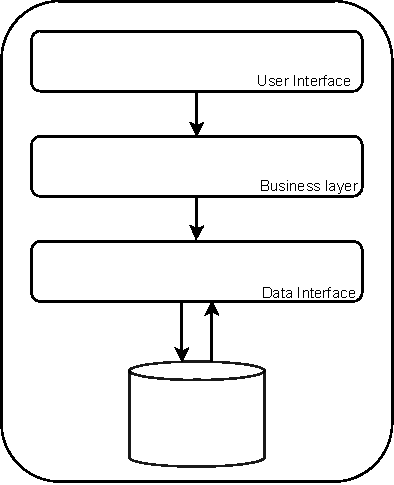
\includegraphics[width=0.3\textwidth]{images/mono.pdf}
    \caption{Monolith Architektur}
    \label{fig:layered-request-flow}
\end{figure}

Einfachere Anwendungen, die diese Architektur nutzen, bieten einige Vorteile. 
Sie ermöglichen eine unkomplizierte Integration von querschnittlichen Belangen 
wie Logging oder Sicherheit, da alle Komponenten in derselben Anwendung laufen. 
Ein weiterer Vorteil ist die Reduzierung des Betriebsaufwands, da nur eine 
zentrale Anwendung deployed und betrieben werden muss. \cite{mono2}[S. 1]

Nachteile entstehen jedoch, wenn die Anwendung tatsächlich sehr groß und komplex 
wird. In diesem Fall kann die Komplexität und Unübersichtlichkeit des Code-Bases 
die Weiterentwicklung erschweren und Bugfixes behindern. \cite{mono}[S. 466]\\


\begin{figure}[h!]
    \centering
    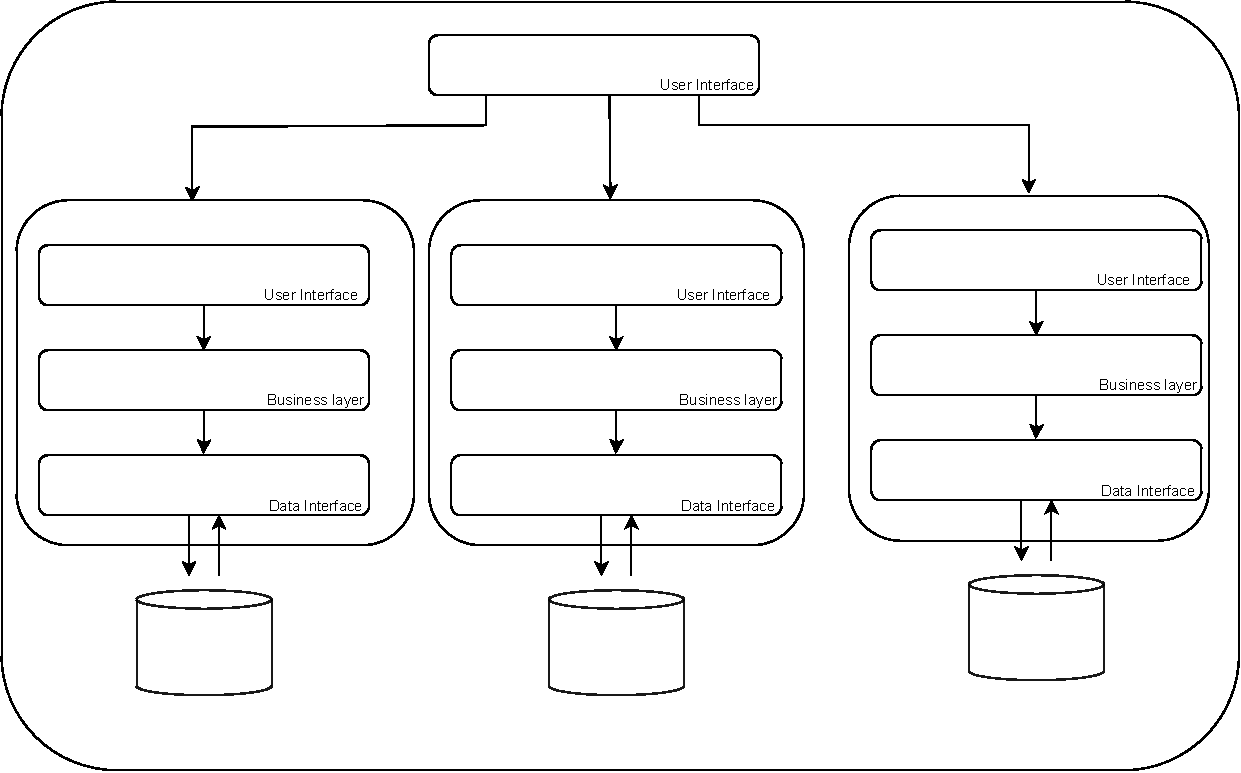
\includegraphics[width=0.5\textwidth]{images/mono-modular.pdf}
    \caption{Modular Monolith Architektur}
    \label{fig:layered-request-flow}
\end{figure}


\subsection{Service-oriented}

Als nächstes wird der Service-oriented Achitektur (SOA) vorgestellt. Ein 
zentrales Konzept sind Services. Ein Service kapselt eine isolierte 
Funktion die über eine definierte Schnittstelle interagiert \cite{soa}[S. 3].
Dieses kann aus einer Reihe von Komponenten bestehen, die gemeinsam eine 
bestimmte Funktionalität bereitstellen. Der Zugriff auf den Service erfolgt über
das Netzwerk, typischerweise mithilfe eines Namens oder eines Locators \cite{soa2}[S. 3].

\section{Fallstudien und Praxisbeispiele}
Blah \ldots \cite{dummy}

\section{Diskussion}

\section{Zusammenfassung und Ausblick}
%(Überblick über die gesamte Arbeit, Rückführung auf Aussagen aus Kapitel 1 durchführen, offene Punkte als neue Forschungsfragen definieren)

\bibliographystyle{ACM-Reference-Format}
\bibliography{sample-base}

\appendix

\section{Anhang 1}

\subsection{Übungsaufgaben}
Blah \ldots

\section{Anhang 2}
Blah \ldots

\end{document}
\endinput
